% !TeX spellcheck = en_US
% !TeX encoding = UTF-8
\chapter{Theoretical foundation}

\section{Stress Measurement}
\subsection{The Stress Response: Physiology of Stress}
\subsection{Photoplethysmogram-PPG}

Photoplethysmogram (PPG) also known as  Blood Volume Pulse (BVP) are non-invasive optical techniques used to monitor changes in blood volume within tissue. They rely on the principles of light absorption and reflection to capture valuable information about cardiovascular activity. PPG and BVP sensors are commonly found in wearable devices. PPG signals are obtained by transmitting light into the skin and measuring the amount of light either transmitted through or reflected back. 

When the heart beats, it propels blood through the circulatory system, causing periodic changes in the volume of blood vessels. PPG sensors emit light into the tissue and measure the amount of light that is either absorbed or reflected back. During each heartbeat, blood absorbs more light, leading to a decrease in the amount of light detected by the sensor. Between heartbeats, when blood flow is less pulsatile, more light is detected.

The resulting waveforms from both PPG and BVP typically consist of a series of peaks and troughs, with each peak corresponding to a heartbeat (systole) and each trough representing the resting period between beats (diastole). By analyzing the time intervals between these peaks, the heart rate can be calculated. This heart rate measurement is fundamental and provides valuable information about a person's cardiovascular health and overall fitness level. It serves as a key metric in various applications, including exercise tracking, stress assessment, and medical diagnosis.

Furthermore, PPG signals enable the assessment of heart rate variability (HRV). HRV is the variation in time between successive heartbeats and is an essential indicator of the autonomic nervous system's activity. By analyzing the subtle changes in the intervals between PPG peaks, HRV can be quantified. High HRV typically indicates a healthy heart and a well-balanced autonomic nervous system, while reduced HRV can be associated with stress, illness, or various medical conditions. HRV analysis provides insights into the body's ability to adapt to different situations and is valuable for assessing stress levels, mental well-being, and overall cardiovascular health.

Other measures that can be derived from PPG data include  and estimation of blood oxygen saturation levels (SpO2), valuable for respiratory and circulatory health assessment. PPG can also be used to estimate respiration rate, reveal vasomotor activity changes associated with the autonomic nervous system, emotions, or vascular health, and provide insights into arterial stiffness and blood flow dynamics. First derivative and second derivates of PPG signals can also be analaysed. The first derivative (Velocity Plethysmogram, VPG) and the second derivative (Acceleration Plethysmogram, APG) features can be used for  blood pressure estimation etc.\parencite{apg}



PPG not only provides heart rate data but, when analyzed, can also reveal heart rate variability (HRV), which is indicative of the body's stress and relaxation levels.

\begin{figure}[h]
    \centering
    % First image
    \begin{subfigure}[b]{0.55\columnwidth}
        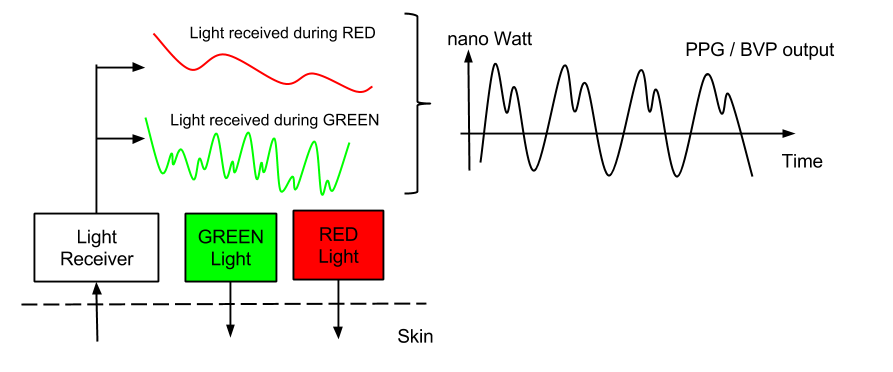
\includegraphics[width=\textwidth]{images/PPG.png}
        \caption{PPG process}
        \label{fig:ppg}
    \end{subfigure}
    % Second image
    \begin{subfigure}[b]{0.35\columnwidth}
        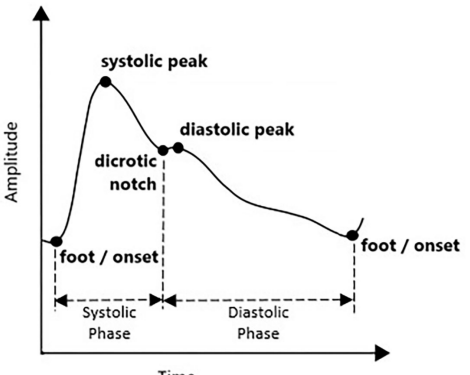
\includegraphics[width=\textwidth]{images/ppg2.png}
        \caption{Typical PPG Waveform}
        \label{fig:phone2}
    \end{subfigure}
    \caption{\parencite{emp} \parencite{apg}}
    \label{fig:phone}
\end{figure}



\subsection{Electrodermal Activity-EDA}
\label{subsec:EDAtheory}

Electrodermal Activity (EDA), also known as the galvanic skin response(GSR), is a way to measure changes in how our skin conducts electricity. Even moderate amounts of sweating that are not observable at the skin surface can alter skin electrical conductivity. The more the body sweats, the more conductive the skin becomes, and this change can be measured to infer physiological or psychological states.More specifically  EDA measures the skin's electrical conductance changes, which depend on the quantity of sweat secreted by eccrine sweat glands in the hypodermis of the palmar and plantar regions. Sweat secreted in the palmar and plantar regions is caused mainly by central nervous activity related to affective and cognitive states, including mental or emotional sweating. Thus EDA becomes one of the promising noninvasive methods widely used in detecting stress and emotion. EDA is a powerful method for real-time measurement and could be used as an index of emotional or cognitive stimulation related to stress.\parencite{gellman2020behavioral}.EDA is useful in several ways: it shows how we respond emotionally, helps us see how our body reacts to stress etc. It acts as a biomarker for emotional responsiveness and serves as a key indicator for stress-related bodily responses. 

Electrodermal Activity (EDA) comprises two main components: the tonic and phasic components. The tonic component, also known as skin conductance level (SCL), reflects slow and consistent changes in the signal's background. In contrast, the phasic components, referred to as skin conductance response (SCR) or spontaneous fluctuation of skin response, are the rapid and momentary fluctuations within the signal that occur within specific time intervals \parencite*{hernando2017feature}. SCR appears in response to stimuli activating the sympathetic nervous system. Consequently, SCR can be linked to a stimulus and can be valuable in measuring cognitive stress levels. However, directly extracting the components of EDA isn't straightforward.

When EDA sensors measure skin conductivity (SC) signals, they typically yield results in microsiemens. To extract the SCL and SCR components accurately, it is necessary to deconvolve the SC signals \parencite[postnote]{alexander2005separating}. Without proper separation of the original SC signals, overlapping SCRs can lead to less precise information during feature extraction . Therefore, it is crucial to perform deconvolution to distinguish the SCR and SCL signals effectively.

\begin{figure}[hb]
	\centering
	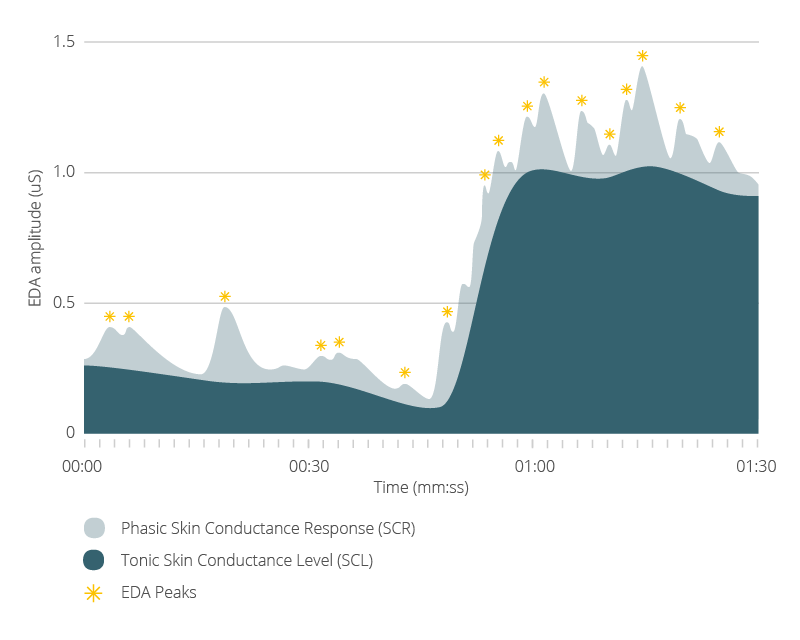
\includegraphics[width=\columnwidth]{images/EDA-example-graph.png}
	\caption{EDA Example signal - \parencite{eda}}
	\label{fig:eda sig}
\end{figure}

\subsection{Empatica E4}
For all the physiological signals explained above, we use the the Empatica E4:
The Empatica E4 wristband is a versatile and compact device designed to capture a wide range of physiological data in real-time. Equipped with sensors for measuring metrics like heart rate, skin conductance, temperature, and motion. Its sleek and unobtrusive nature makes it comfortable to wear, while its comprehensive data collection capabilities have made it an invaluable asset.

The Empatica E4 wristband collects photoplethysmography (PPG) data using a process that involves emitting green and red light from LEDs into the skin and measuring the reflected light with a sensor. The green light, which is absorbed by the blood, provides a pulsatile signal corresponding to the cardiovascular pulse wave, used to determine heartbeats. The red light acts as a reference to correct for motion artifacts. This data is then processed by algorithms within the wristband to output the blood volume pulse (BVP), from which the interbeat interval (IBI)—the time between heartbeats—is calculated, offering a non-invasive method to monitor heart rate continuously.

Electrodermal Activity (EDA) is  measured  by detecting the electrical conductance across the skin, which is an indirect indicator of the sweat gland activity influenced by the sympathetic nervous system. To obtain these measurements, Empatica employs a method that relies on passing a very small and  electrical current between two electrodes that are in contact with the skin, typically placed on the bottom wrist.

The Empatica E4 combines these measurements with additional sensors that track body temperature and movement, providing a comprehensive overview of the wearer's physiological state. This approach allows for a more advanced understanding of the wearer's health, offering potential applications in medical research, clinical trials, and personal health monitoring.


\begin{figure}[hb]
	\centering
	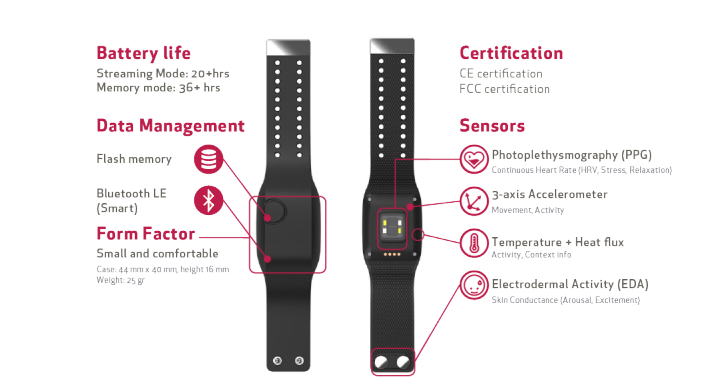
\includegraphics[width=\columnwidth]{images/Empatica.png}
	\caption{Empatica E4 features \parencite{emp}}
	\label{fig:empatica}
\end{figure}


https://support.empatica.com/hc/en-us/articles/204954639-Utilizing-the-PPG-BVP-signal
https://support.empatica.com/hc/en-us/articles/360029719792-E4-data-BVP-expected-signal
%https://box.empatica.com/documentation/20141119_E4_TechSpecs.pdf

\subsection{Motion Capture}
\begin{figure}[h]
    \centering
    % First image
    \begin{subfigure}[b]{0.45\columnwidth}
        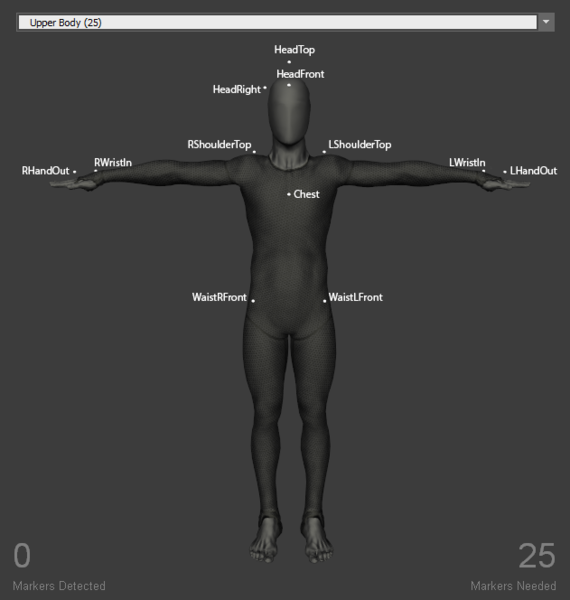
\includegraphics[width=\textwidth]{images/skleton.png}
        \caption{Front View }
        \label{fig:phone1}
    \end{subfigure}
    % Second image
    \begin{subfigure}[b]{0.45\columnwidth}
        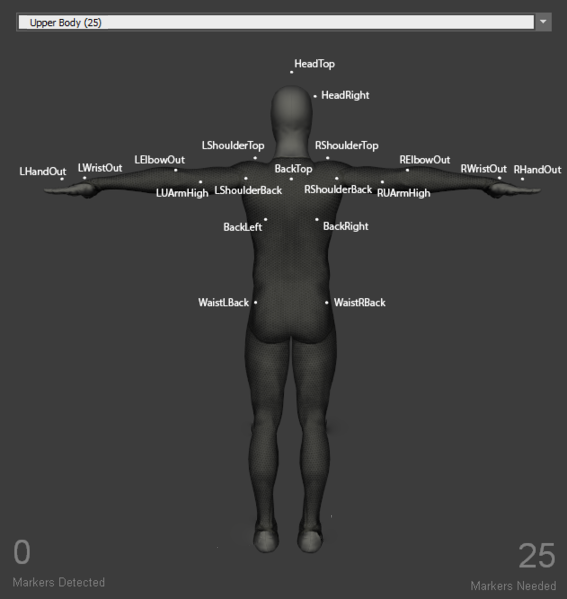
\includegraphics[width=\textwidth]{images/skeleton2.png}
        \caption{Back View }
        \label{fig:phone2}
    \end{subfigure}
    \caption{25 Upper Body Marker Set}
    \label{fig:phone}
\end{figure}

\section{Subjective Measures}
Mental stress can be assessed through subjective and objective
measures. Subjective ratings, such as self-report questionnaires, have
been commonly used to estimate levels of mental stress in humans
(Aigrain et al., 2018). Participants are asked to answer a variety of
questions about their experiences in the experiment. The NASA-Task
Load Index (NASA-TLX) has been utilized in numerous research
studies to assess people’s mental stress levels. For instance, Zheng et al.
(2012) employed the NASA-TLX to investigate the mental workload
experienced by surgeons during endoscopy training. In the context of
smart factories, Zakeri et al. (2021) applied the NASA-TLX to examine
various factors contributing to mental stress, such as task complexity,
time constraints, and collaboration duration. However, it is important to
acknowledge the limitations of self-reporting, as participants cannot
report in real-time and may not express their true feelings (Bethel et al.,
2007). 


\section{UR10 robot and collsion avoidance }


